%----------------------------------------------------------------------------------------
%	PACKAGES AND OTHER DOCUMENT CONFIGURATIONS
%----------------------------------------------------------------------------------------

\documentclass[12pt]{article} % Default font size is 12pt, it can be changed here

\usepackage{geometry} % Required to change the page size to A4
\geometry{a4paper} % Set the page size to be A4 as opposed to the default US Letter

%\usepackage[dutch]{babel} % dutch defaults
\usepackage{graphicx} % Required for including pictures

\usepackage{multirow} \usepackage{rotating} %vertical text in table
 
\usepackage{appendix} 

\usepackage{float} % Allows putting an [H] in \begin{figure} to specify the exact location of the figure
\usepackage{wrapfig} % Allows in-line images such as the example fish picture

\usepackage{lipsum} % Used for inserting dummy 'Lorem ipsum' text into the template

\linespread{1.2} % Line spacing

\setlength\parindent{0pt} % Uncomment to remove all indentation from paragraphs

\graphicspath{{./img/}} % Specifies the directory where pictures are stored

\begin{document}

%----------------------------------------------------------------------------------------
%	TITLE PAGE
%----------------------------------------------------------------------------------------

\begin{titlepage}

\newcommand{\HRule}{\rule{\linewidth}{0.5mm}} % Defines a new command for the horizontal lines, change thickness here

\center % Center everything on the page

\HRule \\[0.4cm]
{ \huge \bfseries Title}\\[0.4cm]
\HRule \\[1.5cm]

\begin{minipage}{0.4\textwidth}
\begin{flushleft} \large
\emph{Auteur:}\\
Roel \textsc{Blaauwgeers}
\end{flushleft}
\end{minipage}
~
\begin{minipage}{0.4\textwidth}
\begin{flushright} \large
\emph{Opdrachtgever:} \\
 \textsc{Opdrachtgever b.v.}
\end{flushright}
\end{minipage}\\[4cm]

{\large \today}\\[3cm] 


\vfill % Fill the rest of the page with whitespace

\end{titlepage}

%----------------------------------------------------------------------------------------
%	TABLE OF CONTENTS
%----------------------------------------------------------------------------------------
%\renewcommand{\contentsname}{Inhoud}
\tableofcontents % Include a table of contents

%\newpage % Begins the essay on a new page instead of on the same page as the table of contents

%let let every section start at a new page
\let\stdsection\section  
\renewcommand\section{\newpage\stdsection}   

%----------------------------------------------------------------------------------------
%	Section 1
%----------------------------------------------------------------------------------------
\section{Section}
\subsection{Subsection1}
Look at table \ref{tab:OS}.
\begin{table}[ht]
\begin{tabular}{|c|c|} \hline
	Android 				& 59.0\%	\\ \hline
	IOS						& 23.0\%	\\ \hline
	Symbian 				& 6.8\%	\\ \hline
	BlackBerry OS 			& 6.4\%	\\ \hline
	Windows Phone/Mobile 	& 2.2\%	\\ \hline
	Andere 					& 2.6\%	\\ \hline
\end{tabular}
	\caption{Mobile OS market share. (IDC Worldwide Mobile Phone Tracker, 24 May, 2012)}
	\label{tab:OS}
\end{table}

\subsection{Subsection2}
Full width image:\\
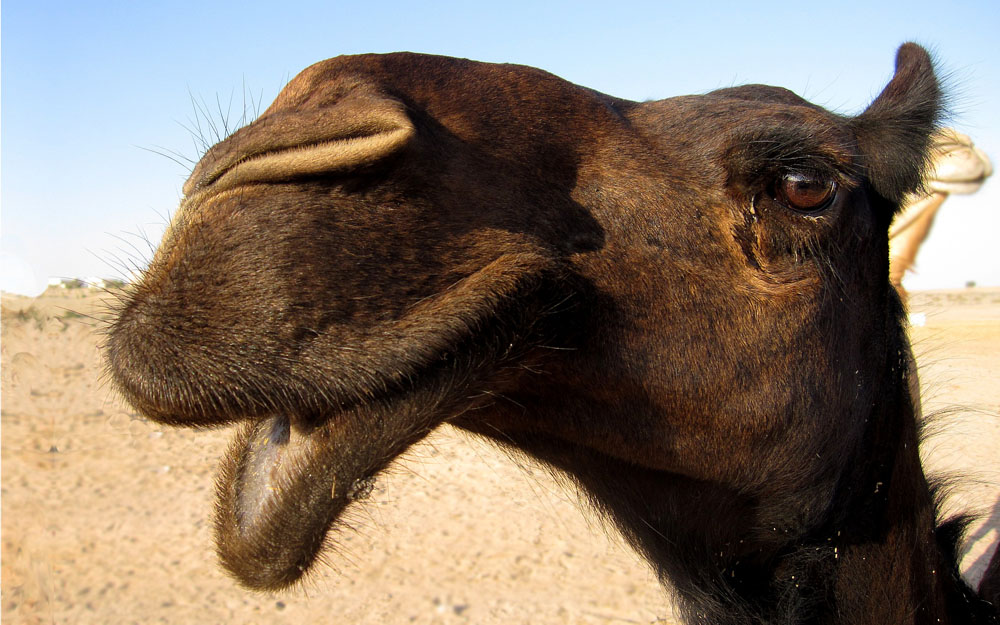
\includegraphics[width=\textwidth]{camel}

\subsection{Subsection3}
This is a \LaTeX~template\cite{bibitem1}.


%----------------------------------------------------------------------------------------
%	BIBLIOGRAPHY
%----------------------------------------------------------------------------------------
%\renewcommand{\refname}{Bronnen}
\begin{thebibliography}{99}
\bibitem{bibitem1}
  Item One,\\
  \emph{http://somedomain.com}
\end{thebibliography}




%----------------------------------------------------------------------------------------
%	APPENDICES
%----------------------------------------------------------------------------------------

\begin{appendices}
	\section{Appendix 1}
	
\end{appendices}
%----------------------------------------------------------------------------------------

\end{document}
